\documentclass[10pt,letterpaper]{article}
%% Welcome to Overleaf!
%% If this is your first time using LaTeX, it might be worth going through this brief presentation:
%% https://www.overleaf.com/latex/learn/free-online-introduction-to-latex-part-1

%% Researchers have been using LaTeX for decades to typeset their papers, producing beautiful, crisp documents in the process. By learning LaTeX, you are effectively following in their footsteps, and learning a highly valuable skill!

%% The \usepackage commands below can be thought of as analogous to importing libraries into Python, for instance. We've pre-formatted this for you, so you can skip right ahead to the title below.

%% Language and font encodings
\usepackage[spanish,english]{babel}
\usepackage[utf8x]{inputenc}
\usepackage[T1]{fontenc}

%% Sets page size and margins
\usepackage[a4paper,top=3cm,bottom=2cm,left=3cm,right=3cm,marginparwidth=1.75cm]{geometry}

%% Useful packages
\usepackage{amsmath}
\usepackage{graphicx}
\usepackage[colorinlistoftodos]{todonotes}
\usepackage[colorlinks=true, allcolors=blue]{hyperref}
\usepackage{algorithm}  
\usepackage{algpseudocode}  
\usepackage{amsmath}  
\renewcommand{\algorithmicrequire}{\textbf{Input:}}  % Use Input in the format of Algorithm  
\renewcommand{\algorithmicensure}{\textbf{Output:}} % Use Output in the format of Algorithm  
\usepackage{listings}
\usepackage{float}
\usepackage{multirow}

 \lstset{ %
    language=Octave,                % the language of the code
    basicstyle=\footnotesize,           % the size of the fonts that are used for the code
    numbers=left,                   % where to put the line-numbers
    numberstyle=\tiny\color{gray},  % the style that is used for the line-numbers
    stepnumber=2,                   % the step between two line-numbers. If it's 1, each line 
                                    % will be numbered
    numbersep=5pt,                  % how far the line-numbers are from the code
    backgroundcolor=\color{white},      % choose the background color. You must add \usepackage{color}
    showspaces=false,               % show spaces adding particular underscores
    showstringspaces=false,         % underline spaces within strings
    showtabs=false,                 % show tabs within strings adding particular underscores
    frame=single,                   % adds a frame around the code
    rulecolor=\color{black},        % if not set, the frame-color may be changed on line-breaks within not-black text (e.g. commens (green here))
    tabsize=2,                      % sets default tabsize to 2 spaces
    captionpos=b,                   % sets the caption-position to bottom
    breaklines=true,                % sets automatic line breaking
    breakatwhitespace=false,        % sets if automatic breaks should only happen at whitespace
    title=\lstname,                 % show the filename of files included with \lstinputlisting;
                                    % also try caption instead of title
    keywordstyle=\color{blue},          % keyword style
    commentstyle=\color{dkgreen},       % comment style
    stringstyle=\color{mauve},         % string literal style
    escapeinside={\%*}{*)},            % if you want to add LaTeX within your code
    morekeywords={*,...}               % if you want to add more keywords to the set
}

%% Title
\title{
		%\vspace{-1in} 	
		\usefont{OT1}{bch}{b}{n}
		\normalfont \normalsize \textsc{CS303 Artifical Intelligence} \\ [10pt]
		\huge Report for NCS Project \\
}

\usepackage{authblk}

\author[1]{Hu yubin, 11712121}

\affil[1]{\small{Department of Computer Science and Engineering, Southern University of Science and Technology}}

\begin{document}
\maketitle

\selectlanguage{english}
\begin{abstract}
NCS is a population-based search algorithm (like genetic algorithm) for continuous optimization problems. The difference is that NCS uses the idea of negatively correlated search to make individuals search different regions in the decision space. This project is to find the best parameter values (i.e. parameter tuning) as you can for NCS on two benchmark test functions (F6 and F12) and one application problem (OLMP).
\end{abstract} \\ 
\\ 
{\textbf{Keywords} \\
NCS, Population-based Search}

\section{Algorithm description}

\subsection{Main Idea of NCS}

\paragraph{}
Negatively correlated search (NCS) maintains multiple individual search processes in parallel and models the search behaviors of individual search processes as probability distributions\cite{Ke2016Negatively}. NCS explicitly promotes negatively correlated search behaviors by encouraging differences among the probability distributions (search behaviors). By this means, individual search processes share information and cooperate with each other to search diverse regions of a search space, which makes NCS a promising method for nonconvex optimization. The co-operation scheme of NCS could also be regarded as a novel diversity preservation scheme that, different from other existing schemes, directly promotes diversity at the level of search behaviors rather than merely trying to maintain diversity among candidate solutions. Empirical studies showed that NCS is competitive to well-established search methods in the sense that NCS achieved the best overall performance on 20 multimodal (nonconvex) continuous optimization problems. The advantages of NCS over state-of-the-art approaches are also demonstrated with a case study on the synthesis of unequally spaced linear antenna arrays.

\paragraph{}
In other words, NCS aims to control each search agent to search the part of the search space that other search agents will not search.
\begin{itemize}
    \item 
    NCS first calculates the negative correlation (i.e. search behavior diversity) between different search agents
\end{itemize}
\begin{itemize}
    \item 
    Then, selects the search agents that have higher negative correlation with other search agents.
\end{itemize}

\paragraph{}
We don't want two agents search the similar region like the left chart in Figure 1, so we wish distributions have the large distance like the right chart in Figure 1.
\begin{figure}[H]
  \centering
  % Requires \usepackage{graphicx}
  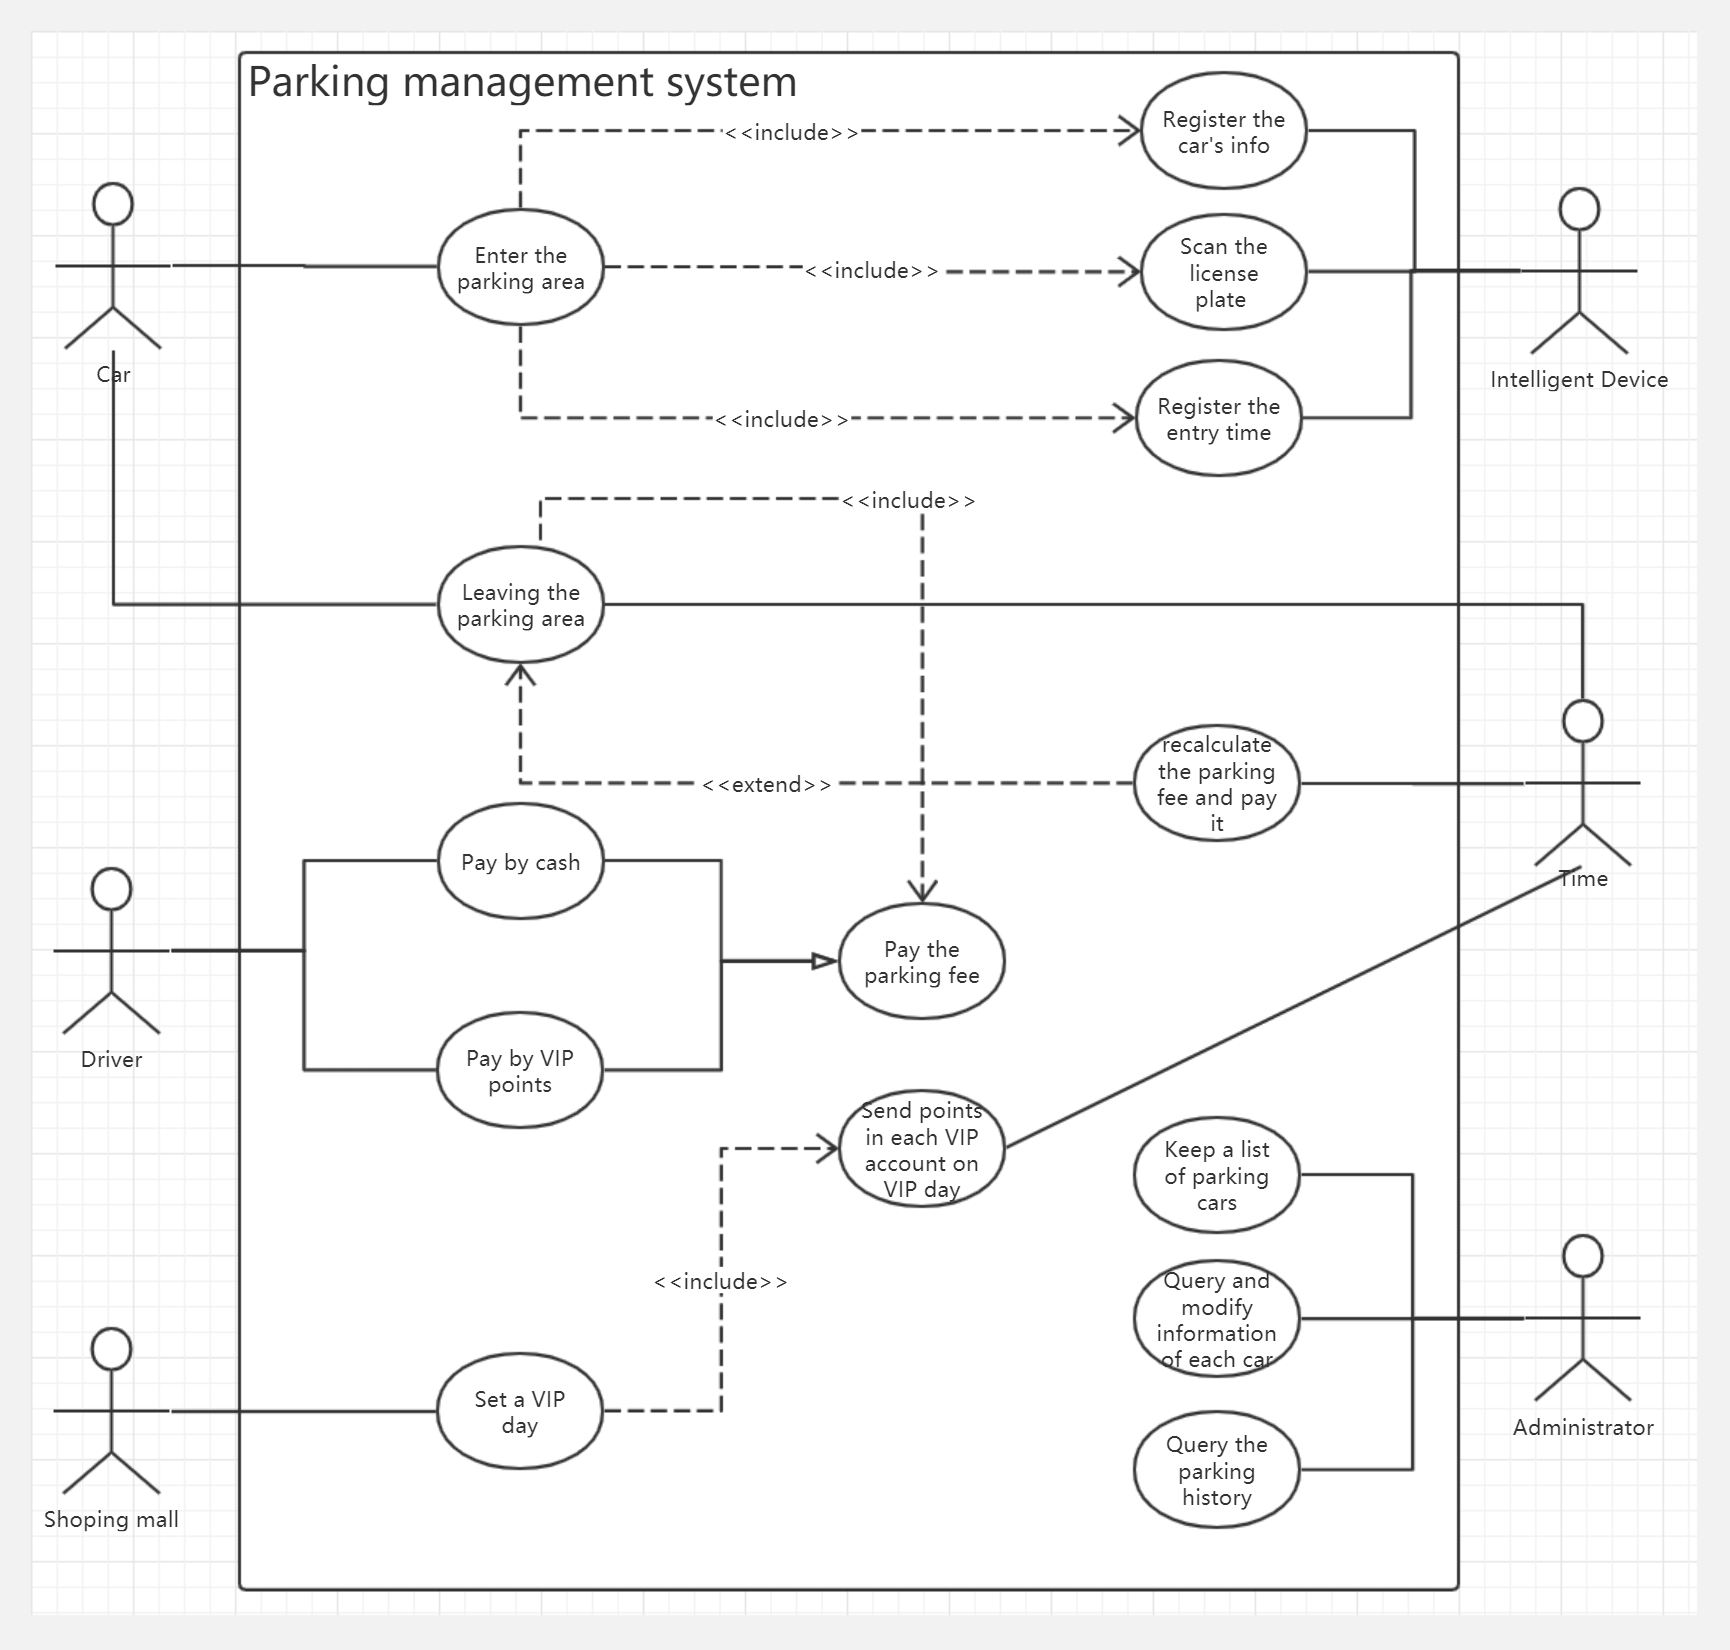
\includegraphics[width=0.8\textwidth]{Fig1.png}\\
  \caption{Distance between distributions}
  \label{straddltimeScale}
\end{figure}

\paragraph{}
There are many metrics for measuring the distance between distributions, NCS adopts the Bhattacharyya distance. 
\begin{itemize}
    \item 
    For continuous case: $D_B(p_i,P_j) = -\ln (\int\sqrt{p_i(x)p_j(x)}dx)$
\end{itemize}
\begin{itemize}
    \item 
    For discrete case: $D_B(p_i,P_j) = -\ln (\sum_{x{\in}X}\sqrt{p_i(x)p_j(x)})$
\end{itemize}
In case of $N(N>2)$ agents, the distance of a distribution $p_i$ to the other distributions is measured as: $Corr(p_i) = min{D_B(p_i,p_j)|j{\neq}i}$

\paragraph{}
Not only search behavior diversity (i.e. distribution distance), should also care about whether the search agent can find a better solution. We want to find the solution with both high fitness and large distance. The following heuristic is adopted to control the trade-off between two criteria: \\
where λ>0 is a parameter
\begin{cases}
    \mathcaldiscard $x_i$, &\text{if $\frac{f(x_i')}{Corr(p_i')}<\lambda$}\\
	\mathcaldiscard $x_i'$, &\text{if $otherwise$}
\end{cases}
  
\paragraph{}
Now, we discuss a simple instantiation of NCS, namely NCS-C is implemented to demonstrate the effectiveness of NCS on continuous multimodal optimization problems. We generate the $x_{id}'$ by $x_{id}$ with Gaussian mutation operator.
$$x_{id}'=x_{id}+\mathcal{N}(0,\sigma_i)$$

\paragraph{}
To keep the algorithm simple, all RLSs in NCS-C are initialized with the same value of σi . Then, each σi is adapted for every epoch iterations according to the 1/5 successful rule suggested\cite{Beyer2002Evolution}\\
$\sigma_i=$
\begin{cases}
    \mathcaldiscard $\frac{\sigma_i}{r}$, &\text{if $\frac{x}{epoch}>0.2$}\\
	\mathcaldiscard $\sigma_i*r$, &\text{if $\frac{x}{epoch}<0.2$}\\
	\mathcaldiscard $\sigma_i$, &\text{if $\frac{x}{epoch}=0.2$}
\end{cases}\\
where $r$ is a parameter that is suggested to be set beneath 1, and $c$ is the times that a replacement happens (i.e., $x_i'$ is preserved) during the past epoch iterations. Equation is designed based on the following intuition. A large $c$ implies that the RLS frequently found better solutions in the past iterations, and the current best solution might be close to the global optimum. Thus, the search step-size should be reduced (by $r$ times). On the other hand, if a RLS frequently failed to achieve a better solution in the past iterations, it might have been stuck in a local optimum. In this case, the search step-size will be increased (by r times) to help the RLS explore other promising regions in the search space.

\paragraph{}
The above is the main idea of the NCS algorithm, the following is the pseudo code of this algorithm.
\begin{figure}[H]
  \centering
  % Requires \usepackage{graphicx}
  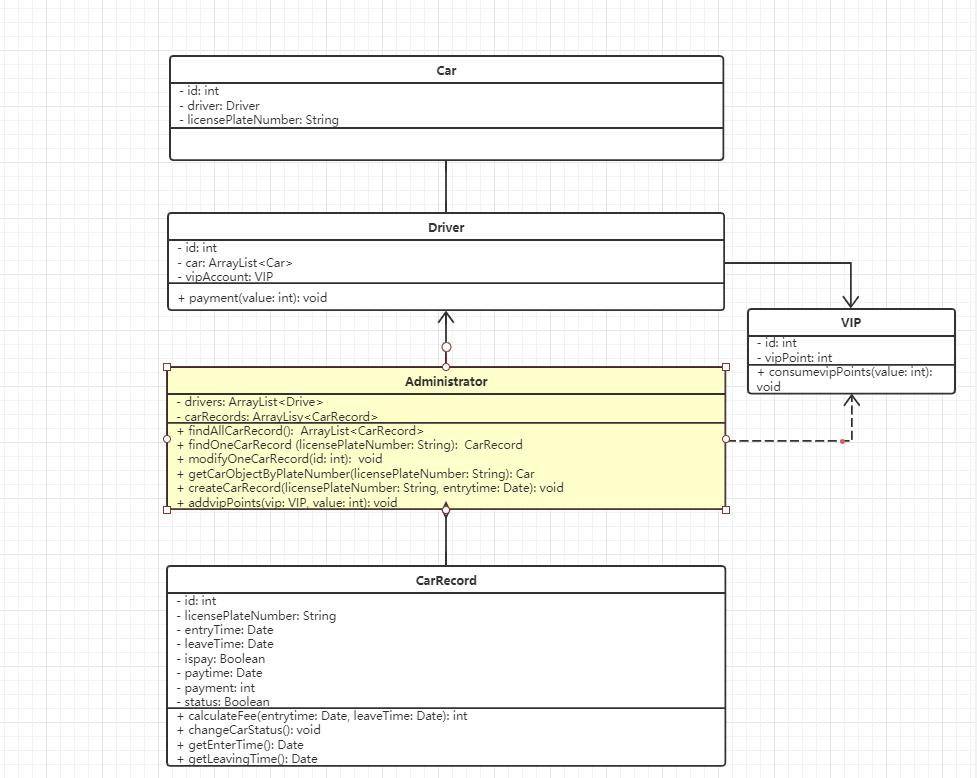
\includegraphics[width=0.8\textwidth]{Fig2.png}\\
  \caption{Pseudo code of NCS alorithm}
  \label{straddltimeScale}
\end{figure}

\subsection{Applications of NCS}

\paragraph{}
The application of a communication system often requires solving a challenging optimization problem. For example, minimizing the Symbol-Error-Rate (SER) for Amplify-and-Forward Relaying Systems is nontrivial since the SER surface is non-convex and has multiple minima\cite{Ahmed2015Minimizing}. When tuning the protocol of sensornets\cite{TateEvolutionary}, as mathematical modeling of sensornets involves numerous inherent difficulties, one might has to deal with the optimization problem without an explicit objective function and the quality of candidate protocol configurations could only be obtained from a simulation model. In the era of Big Data, as data analytics (e.g., machine learning) fast grows into a ubiquitous technology in many areas, including communications, the challenges brought by complex optimization problems become even more important than ever.

\paragraph{}
First, one of the major roles of big data analytics is to acquire knowledge from data in order to facilitate decision-making, e.g., managing network resources based on the analysis of user profiles to achieve higher endusers satisfaction. Thus, the value of big data usually needs to be created through tackling an optimization problem (i.e., to seek the optimal decision), which is formulated based on the knowledge obtained from big data analytics. Such optimization problems may not only be non-convex, but also be noisy due to the noise contained in the original data. Furthermore, the data analytics process may also involve complex optimization problems, such as training deep neural networks or tuning the hyper-parameter of Support Vector Machines. To cope with these complex optimization problems, Evolutionary Algorithms (EAs) have been widely adopted and been shown to be a family of powerful tools. In short, to create business values from big data analytics, optimization tools are indispensable.

\subsection{Main Idea of OLMP}

\paragraph{}
Layer-wise magnitude-based pruning (LMP) is a very popular method for deep neural network (DNN) compression. However, tuning the layerspecific thresholds is a difficult task, since the space of threshold candidates is exponentially large and the evaluation is very expensive. Previous methods are mainly by hand and require expertise. In this paper, we propose an automatic tuning approach based on optimization, named OLMP. The idea is to transform the threshold tuning problem into a constrained optimization problem (i.e., minimizing the size of the pruned model subject to a constraint on the accuracy loss), and then use powerful derivative-free optimization algorithms to solve it. To compress a trained DNN, OLMP is conducted within a new iterative pruning and adjusting pipeline. Empirical results show that OLMP can achieve the best pruning ratio on LeNet-style models (i.e., 114 times for LeNet-300-100 and 298 times for LeNet-5) compared with some state-ofthe-art DNN pruning methods, and can reduce the size of an AlexNet-style network up to 82 times without accuracy loss.

\paragraph{}
Layer-wise magnitude-based pruning (LMP) is an effective DNN compression method and has achieved significant results in many applications. The idea is to prune connections in each layer separately by removing the connections with absolute weight values lower than a layer-specific threshold. Given a threshold for each layer, LMP can prune connections in parallel, which is especially useful for DNNs with millions or billions connections. With well chosen pruning thresholds, LMP can achieve a significant reduction in the number of parameters, while maintaining a relatively low accuracy loss.

\paragraph{}
However, if the parameters of the LMP are manually adjusted, it is difficult to adjust the optimal parameters and it takes a lot of time and cost. So that the proposed OLMP adopts a heuristic optimization algorithm NCS\cite{Ke2016Negatively} to optimize the pruning thresholds. Heuristic optimization algorithms have been used to evolve the network structure, and to prune the connections. However, most of them are effective only for shallow networks, and are computational impossible for DNNs with millions of parameters.

\begin{figure}[H]
  \centering
  % Requires \usepackage{graphicx}
  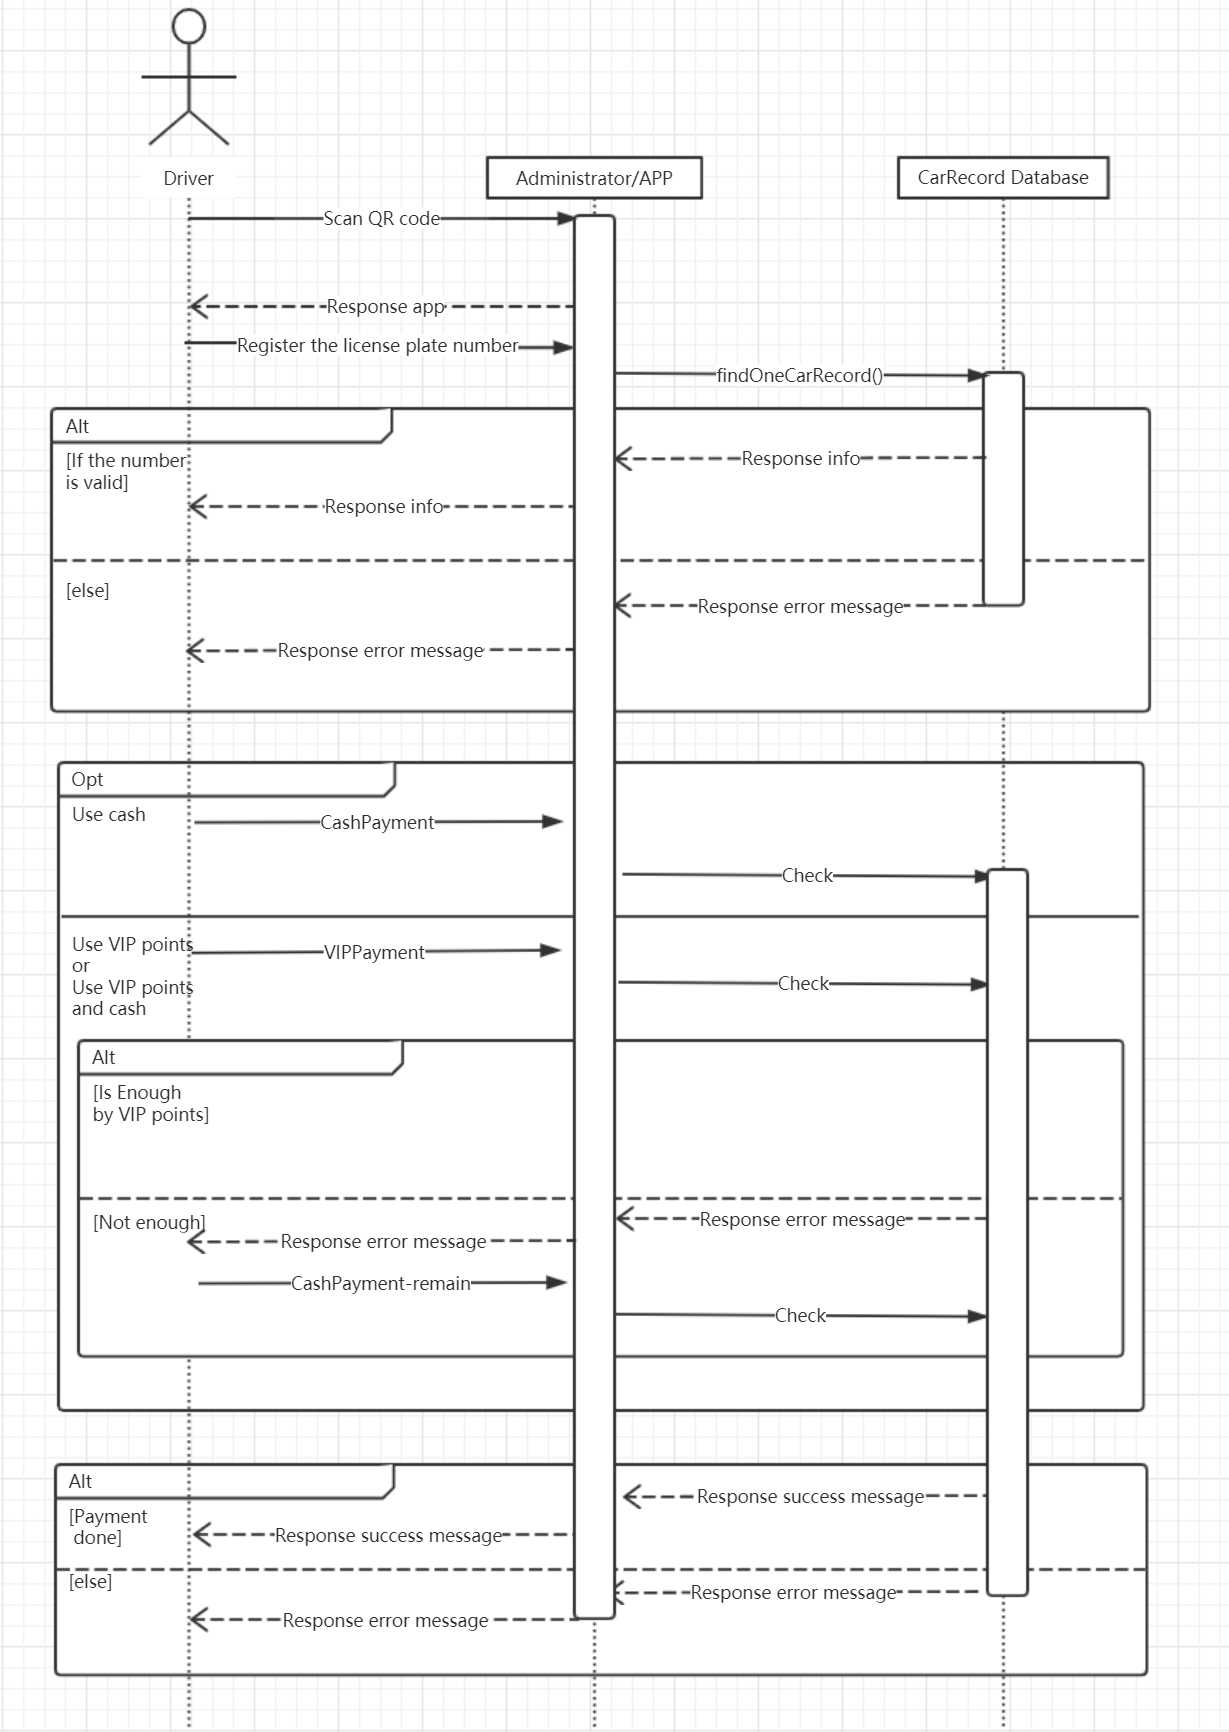
\includegraphics[width=0.8\textwidth]{Fig3.png}\\
  \caption{Illustration of DNN compression with OLMP, given an accuracy constraint δ, and a reference model as inputs. The \emph{Right part} presents the compression process in which pruning and adjusting are conducted iteratively until the stopping criterion is fulfilled. The pruning step adopts OLMP to generate a pruned model, while the adjusting step recovers the accuracy loss of the pruned model. In each loop of pruning and adjusting, it will fetch a small set of data with K batches from the whole data set D, and use one batch for pruning while the rest for adjusting. The \emph{Left part} illustrates the structure of OLMP using NCS. In OLMP, the threshold tuning problem is formulated as a single-objective optimization problem with an accuracy constraint δ, and then optimized using NCS to get the best found thresholds. After that, a pruned model can be derived by applying LMP on the reference model with the obtained thresholds.}
  \label{straddltimeScale}
\end{figure}

\subsection{Applications of OLMP}

\paragraph{}
Without incurring any accuracy loss on test data, OLMP can prune 99.66\% parameters of LeNet-5 and 99.12\% parameters of LeNet-300-100, which are the best results in comparison to a number of state-of-the-art approaches. Prof.Tang apply OLMP to prune an AlexNet-style deep model and 98.78\% parameters can be removed without sacrificing accuracy.\cite{li2018optimization}

\paragraph{}
Recently, Google Research successfully applied genetic algorithms to design the structures of DNNs by using clusters of GPU servers.

\section{Parameter description}

\begin{table}[H]
\begin{tabular}{|c|c|c|c|}
\hline
\multirow{2}{*}{\textbf{Parameters}} & \multicolumn{3}{c|}{\textbf{Your final values and results}} \\ \cline{2-4} 
                                     & \textbf{F6}        & \textbf{F12}      & \textbf{OLMP}      \\ \hline
\textbf{lambda}                      & 1.1894114828452    & 0.992687616933805 & 6                  \\ \hline
\textbf{r}                           & 0.524759241553746  & 0.569352821038384 & 0.1999             \\ \hline
\textbf{epoch}                       & 8                  & 114               & 10                 \\ \hline
\textbf{n}                           & 1                  & 1                 & 92                 \\ \hline
\textbf{Final Result}                & 390.00000000000347 & -460              & 0.9889914106747684 \\ \hline
\textbf{Running Time}                & 47.61029505729675  & 34.49642562866211 & 62.54827380180359  \\ \hline
\end{tabular}
\end{table}

\begin{itemize}
    \item \emph{Summary}
    \begin{itemize}
        \item \emph{lambda}
        \begin{itemize}
            \item \emph{role}\\
            Not only search behavior diversity (i.e. distribution distance), should also care about whether the search agent can find a better solution. We want to find the solution with both high fitness and large distance. The following heuristic is adopted to control the trade-off between two criteria: \\
            where λ>0 is a parameter
            \begin{cases}
                \mathcaldiscard $x_i$, &\text{if $\frac{f(x_i')}{Corr(p_i')}<\lambda$}\\
            	\mathcaldiscard $x_i'$, &\text{if $otherwise$}
            \end{cases}\\
            In order to balance better fitness and longer distances, there is a coefficient lambda
        \end{itemize}
        \begin{itemize}
            \item \emph{effect}\\
            For F6 and F12, in order to balance better fitness and longer distances, lambda is close to 1. But the specific value of the lambda needs to be decided together with r.\\
            For OLMP, lambda is irrelevant to the answer. The answer is only related to n.
        \end{itemize}
        \begin{itemize}
            \item \emph{best range}\\
            The experimental results show that the value of lambda is between 1.0 and 1.2.
        \end{itemize}
    \end{itemize}
    \begin{itemize}
        \item \emph{r}
        \begin{itemize}
            \item \emph{role}\\
            $r$ is a parameter that is suggested to be set beneath 1, and $c$ is the times that a replacement happens (i.e., $x_i'$ is preserved) during the past epoch iterations. Equation is designed based on the following intuition. A large $c$ implies that the RLS frequently found better solutions in the past iterations, and the current best solution might be close to the global optimum. Thus, the search step-size should be reduced (by $r$ times). On the other hand, if a RLS frequently failed to achieve a better solution in the past iterations, it might have been stuck in a local optimum. In this case, the search step-size will be increased (by r times) to help the RLS explore other promising regions in the search space.
        \end{itemize}
        \begin{itemize}
            \item \emph{effect}\\
            For F6 and F12, when the replacement happens many times, the range of the Gaussian mutation may expand or shrink. r has more effect on answer d than lambda. But the specific value of the lambda needs to be decided together with lambda.\\
            For OLMP, r is irrelevant to the answer. The answer is only related to n.
        \end{itemize}
        \begin{itemize}
            \item \emph{best range}\\
            The experimental results show that the value of r is between 0.4 and 0.6. I think this value is close to 0.5, similar to a binary search.
        \end{itemize}
    \end{itemize}
    \begin{itemize}
        \item \emph{epoch}
        \begin{itemize}
            \item \emph{role}\\
        To keep the algorithm simple, all RLSs in NCS-C are initialized with the same value of σi . Then, each σi is adapted for every epoch iterations according to the 1/5 successful rule suggested\cite{Beyer2002Evolution}\\
        $\sigma_i=$
        \begin{cases}
            \mathcaldiscard $\frac{\sigma_i}{r}$, &\text{if $\frac{x}{epoch}>0.2$}\\
        	\mathcaldiscard $\sigma_i*r$, &\text{if $\frac{x}{epoch}<0.2$}\\
        	\mathcaldiscard $\sigma_i$, &\text{if $\frac{x}{epoch}=0.2$}
        \end{cases}\\
        \end{itemize}
        \begin{itemize}
            \item \emph{effect}\\
            The definition of epoch in deep neural networks is the number of cycles to train the entire training set.\\
            For F6 and F12, if the other three parameters are unchanged, only the epoch is changed, and the answer is different. But if we determine the values of epoch and n, only change lambda and r, we can always get a better solution (error is less than $10^{-10}$).\\
            For OLMP, epoch is irrelevant to the answer. The answer is only related to n.
        \end{itemize}
        \begin{itemize}
            \item \emph{best range}\\
            The experimental results show that the value of epoch is more than 100 is more suitable. Because when the value of epoch is greater than 100, it can appropriately adjust the range of Gaussian mutation to become larger or smaller, while achieving a better local optimal solution.
        \end{itemize}
    \end{itemize}
    \begin{itemize}
        \item \emph{n}
        \begin{itemize}
            \item \emph{role}\\
            For the sake of simplicity, we consider a special case that each search process is a Randomized Local Search (RLS), which produces one new candidate solution in each iteration. In other words, we consider a population-based search method with population size of n(n > 1), which runs n RLS procedures in parallel and iteratively updates each individual solution in the population with a randomized search operator
        \end{itemize}
        \begin{itemize}
            \item \emph{effect}\\
            For F6 and F12, because we run programs through multiple processes, we can run many different sets of parameters randomly, so n is not very important. In order to minimize the number of parameters affecting the result, we assume that n is equal to 1, so that the lambda has no effect on the answer, and we fixed the epoch, so the answer is related to r, so it is easy to climb the mountain algorithm or simulate annealing algorithm obtains the local optimal solution.\\
            For OLMP, n is the only parameter that determines the result.
        \end{itemize}
        \begin{itemize}
            \item \emph{best range}\\
            For F6 and F12, because we run programs through multiple processes, we think n equals 1 is well.
            For OLMP, experiments show that we traverse the range of n (1 to 100), we find that the results are independent of other parameters, and when n is equal to 92, the result is the best.
        \end{itemize}
    \end{itemize}
\end{itemize}

\section{Tuning procedure}

\paragraph{}
For F6 and F12, we first consider the extent to which the four parameters affect the answer. We tested some data and found that regardless of the epoch equal, the other three parameters have a chance to get better results. Because we run programs through multiple processes, we can run many different sets of parameters randomly, so n is not very important. In order to minimize the number of parameters affecting the result, we assume that n is equal to 1, so that the lambda has no effect on the answer, and we fixed the epoch, so the answer is related to r.

\paragraph{}
So we fixed n equal to 1, epoch is an arbitrary positive integer (preferably greater than 100), and the value of lambda is around 0.5. Then we rewrote NCS-client and made it a method that allows us to call multiple processes to get the result. Then we randomly generate the value of r according to the number of cores of our server, and bring the parameters into the rewritten NCS-client or the result. We know that the minimum value of F6 is 390, and the minimum value of F12 is -460. Therefore, we select the parameters of the previous random parameters whose results are close to the minimum value to run a further optimization algorithm.

\begin{figure}[H]
  \centering
  % Requires \usepackage{graphicx}
  \includegraphics[width=0.8\textwidth]{Fig6.png}\\
  \caption{server: We have run 30 processes on this server.}
  \label{straddltimeScale}
\end{figure}

\begin{figure}[H]
  \centering
  % Requires \usepackage{graphicx}
  \includegraphics[width=0.8\textwidth]{Fig8.png}\\
  \caption{hill climbing data}
  \label{straddltimeScale}
\end{figure}

\begin{figure}[H]
  \centering
  % Requires \usepackage{graphicx}
  \includegraphics[width=0.6\textwidth]{Fig4.png}\\
  \caption{F6}
  \label{straddltimeScale}
\end{figure}

\begin{figure}[H]
  \centering
  % Requires \usepackage{graphicx}
  \includegraphics[width=0.6\textwidth]{Fig5.png}\\
  \caption{F12}
  \label{straddltimeScale}
\end{figure}

\paragraph{}
After we have the appropriate parameters, we use the hill climbing algorithm as our optimization algorithm to continue to optimize the parameters. After running for 30 days, we got better results (error is less than $10^{-10}$)

\begin{algorithm}
  \caption{Hill Climbing}
  \begin{algorithmic}[1]
    \Function {Hill-Climbing}{}
        \If {vaild parameter}
            parameter = init()
        \EndIf
        \While{stopping condition is not reached}:
            x' = Gaussian-mutation(x)
            ans = NCS(x)
            ans' = NCS(x')
            \If{ans'<ans}:
                x = x'
            \EndIf
        \EndWhile\\
        \Return x
    \EndFunction  
  \end{algorithmic}  
\end{algorithm}

\paragraph{}
For OLMP, after several random attempts, we were pleasantly surprised to find that the results are not related to lambda, r, epoch, only related to n, so we traversed the range of n (1 to 100) and finally found that when n is equal to 92 At the time, the result is the biggest.

\begin{figure}[H]
  \centering
  % Requires \usepackage{graphicx}
  \includegraphics[width=0.8\textwidth]{Fig7.png}\\
  \caption{Several parameters}
  \label{straddltimeScale}
\end{figure}

\bibliographystyle{ieeetr}
\bibliography{references}

\end{document}
